\documentclass[12pt]{article}

\usepackage{pablo-devoir}
\usepackage[a5paper,margin=2cm]{geometry}

\pagestyle{empty}

\title{\large Fonctions affines Vecteurs}
\date{11/02/15}
\classe{2\up{des}14}
\dsnum{DS 5}

\begin{document}
\textbf{\Large Nom : \ldots\ldots\ldots\ldots\ldots\ldots\ldots\ldots\ldots}
\vspace{.5cm}

\maketitle

\begin{exercice}[Fonctions affines --- 7 points]~
  On considère la fonction affine $f$ passant par les points $A\left( -1;2 \right)$ et $\left( 2;5 \right)$.
  \begin{enumerate}
    \item 
      \begin{enumerate}
        \item Calculer l'équation de la fonction $f$.
        \item La fonction est-elle croissante ou décroissante ?
      \end{enumerate}
    \item 
      \begin{enumerate}
        \item Dresser le tableau de signes de la fonction $g:x\mapsto -2x+8$, définie sur $\mathbb{R}$.
        \item Sans calculer sa valeur, dire si $f(10)$ est positif ou négatif.
      \end{enumerate}
  \end{enumerate}
\end{exercice}

\begin{exercice}[Parallélogramme --- 6 points]
  On considère un parallélogramme $ABCD$, et un point $E$ tel que $C$ soit le
  milieu de $\left[ BE \right]$, comme représentés sur la figure suivante.

  \begin{center}
    \begin{tikzpicture}[very thick, scale=1]
      \coordinate (A) at (1.4, 2);
      \coordinate (B) at (0, 0);
      \coordinate (C) at (2, -.3);
      \coordinate (D) at ($(A)+(C)-(B)$);
      \coordinate (E) at ($2*(C)-(B)$);

      \draw (A) node{$\bullet$} node[above left]{$A$};
      \draw (B) node{$\bullet$} node[below left]{$B$};
      \draw (C) node{$\bullet$} node[below]{$C$};
      \draw (D) node{$\bullet$} node[above right]{$D$};
      \draw (E) node{$\bullet$} node[below right]{$E$};

      \draw (A) -- (B) -- (C) -- (D) -- cycle;
    \end{tikzpicture}
  \end{center}
  \begin{enumerate}
    \item Justifier que $\vecteur{BC}=\vecteur{CE}$.
    \item Quelle est la relation entre $\vecteur{AD}$ et $\vecteur{CE}$ ? Justifier.
    \item En déduire la nature du quadrilatère $ADEC$.
  \end{enumerate}
\end{exercice}

\begin{exercice}[Placer des points --- 7 points]~
  On considère les points $A$, $B$, $C$ suivants.
  \begin{center}
    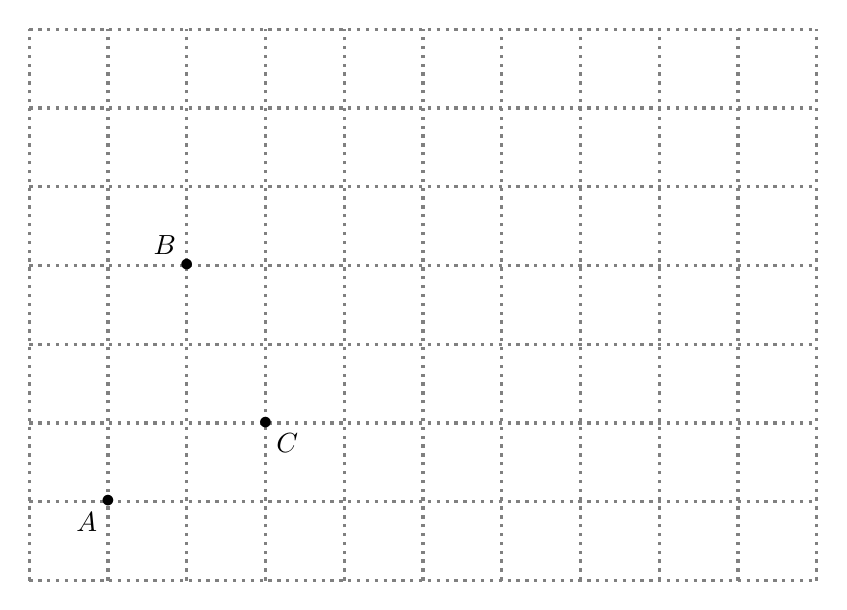
\begin{tikzpicture}[very thick]
      \draw[dotted, gray] (0,0) grid (10,7);
      \draw (1,1) node{$\bullet$} node[below left]{$A$};
      \draw (2,4) node{$\bullet$} node[above left]{$B$};
      \draw (3,2) node{$\bullet$} node[below right]{$C$};
    \end{tikzpicture}
  \end{center}
  \begin{enumerate}
    \item Placer le point $D$ tel que $\vecteur{BD}=2\vecteur{AC}$.
    \item On aimerait placer $E$ tel que $\vecteur{AE}=2\vecteur{CA}+2\vecteur{BD}$, mais placer ce point directement ferait sortir de la feuille. Nous allons faire autrement.
      \begin{enumerate}
        \item Montrer que $\vecteur{CA}+\vecteur{BD}=\vecteur{AC}$.
        \item En déduire que $\vecteur{AE}=2\vecteur{AC}$.
        \item Placer enfin le point $E$.
      \end{enumerate}
  \end{enumerate}

\end{exercice}

\begin{exercice}[Bonus --- 1 points]
  Soient $A$ et $B$ deux points distincts. Lequel des deux vecteurs suivants a
  la plus grande norme : $\vecteur{AB}-\vecteur{BA}$, ou
  $\vecteur{AB}+\vecteur{BA}$ ? Justifier.
\end{exercice}

\end{document}
